% Created 2021-09-22 Wed 14:29
% Intended LaTeX compiler: pdflatex
\documentclass[11pt]{article}
\usepackage[utf8]{inputenc}
\usepackage{lmodern}
\usepackage[T1]{fontenc}
\usepackage[top=1in, bottom=1.in, left=1in, right=1in]{geometry}
\usepackage{graphicx}
\usepackage{longtable}
\usepackage{float}
\usepackage{wrapfig}
\usepackage{rotating}
\usepackage[normalem]{ulem}
\usepackage{amsmath}
\usepackage{textcomp}
\usepackage{marvosym}
\usepackage{wasysym}
\usepackage{amssymb}
\usepackage{amsmath}
\usepackage[theorems, skins]{tcolorbox}
\usepackage[version=3]{mhchem}
\usepackage[numbers,super,sort&compress]{natbib}
\usepackage{natmove}
\usepackage{url}
\usepackage[cache=false]{minted}
\usepackage[strings]{underscore}
\usepackage[linktocpage,pdfstartview=FitH,colorlinks,
linkcolor=blue,anchorcolor=blue,
citecolor=blue,filecolor=blue,menucolor=blue,urlcolor=blue]{hyperref}
\usepackage{attachfile}
\usepackage{setspace}
\usepackage{geometry}
\geometry{margin=1.0in}
\usepackage{outline}
\usepackage{amsmath}
\usepackage{graphicx}
\usepackage{epstopdf}
\usepackage{fancyhdr}
\usepackage{hyperref}
\usepackage[labelfont=bf]{caption}
\setlength{\headheight}{15.2pt}
\def\dbar{{\mathchar'26\mkern-12mu d}}
\pagestyle{fancy}
\fancyhf{}
\renewcommand{\headrulewidth}{0.5pt}
\renewcommand{\footrulewidth}{0.5pt}
\lfoot{\today}
\cfoot{\copyright\ 2021 W.\ F.\ Schneider}
\rfoot{\thepage}
\lhead{\em{Advanced Chemical Reaction Engineering}}
\rhead{ND CBE 60546}
\setcounter{secnumdepth}{3}
\author{William F. Schneider}
\date{\today}
\title{CBE 60546 Outline}
\begin{document}

\begin{OPTIONS}
\end{OPTIONS}
\section{Lecture 0: Intro to Reaction Engineering}
\label{sec:org68ce340}
\begin{enumerate}
\item Reaction engineering
\end{enumerate}
\begin{quote}
Understanding, modeling, designing, using, controlling, analyzing, improving anything in which chemical reactions happen.
\end{quote}
\begin{enumerate}
\item Reaction engineering applications
\begin{enumerate}
\item Traditional
\begin{enumerate}
\item Industrial chemical/petroleum processes
\item Fine chemical/pharmaceutical processes
\item Emerging, eg biorefinergy, shale gas, \url{http://cistar.us}
\end{enumerate}
\item Energy storage, batteries, fuel cells
\item Environmental systems
\begin{enumerate}
\item Atmosphere, lake, bioreactor (water purification), catalytic convertor
\end{enumerate}
\item Biological systems
\begin{enumerate}
\item Cell, organ, body
\end{enumerate}
\item Laboratory reactors - interrogate, quantify
\item Research - improved materials (catalysts), improved processes, understand limitations
\begin{enumerate}
\item Sabatier plot, \url{https://doi.org/10.1038/nchem.121}
\end{enumerate}
\end{enumerate}
\item Course structure
\begin{enumerate}
\item Quantifying chemical reactions
\begin{enumerate}
\item Stoichiometry
\item Thermodynamics - heat flow, direction, equilibrium
\item Kinetics - rates, mechanisms
\end{enumerate}
\item Physical/chemical interactions
\begin{enumerate}
\item Transport, mixing, diffusion resistance, \ldots{}
\end{enumerate}
\item Chemical reactors
\begin{enumerate}
\item Ideal 0 and 1-dimensional
\item Non-ideal
\item Non-isothermal
\item Non-steady state
\item Multiphase
\end{enumerate}
\item Chemical processes (beyond us)
\item Markets (beyond us)
\end{enumerate}
\end{enumerate}

\section{Stoichiometry and reactions}
\label{sec:org07637e3}
\begin{enumerate}
\item Substances
\item Amounts
\begin{enumerate}
\item mass, moles, volumes
\item flow rates
\end{enumerate}
\item compositions
\begin{enumerate}
\item amount/total amount
\end{enumerate}
\item Reactions and stoichiometric coefficients
\begin{enumerate}
\item Advancements \(n_j = \sum_i \nu_{ij} \xi_i\)
\item Limiting reagents
\end{enumerate}
\end{enumerate}
\section{Chemical thermodynamics and equilibria}
\label{sec:orgd8c8f0f}
\begin{enumerate}
\item Chemical reactions \(\sum_j \nu_j A_j = 0\)
\item Thermodynamic potential differences
\begin{enumerate}
\item Standard states
\item Formation reactions
\item Reaction enthalpy \(\Delta H^\circ (T) = \sum_j \vu_j H^\circ_j (T) = \sum_j \nu_j H^\circ_{f,j}(T)\)
\item Reaction entropy \(\Delta S^\circ (T) =  \sum_j \vu_j S^\circ_j (T)\)
\end{enumerate}
\item Equilibrium-closed system
\begin{enumerate}
\item Free energy vs reaction advancement, \(G(\xi,T) = \sum_j n_j\mu_j = \sum_j \left (n_{j0} + \nu_j \xi \right ) \left (\mu_j^\circ(T) + RT \ln a(\xi,T) \right )\)
\item Equilibrium \((\partial G / \partial \xi)_{T,P} = 0\)
\item Equilibrium constants and algebraic solutions
\item Multiple reactions
\end{enumerate}
\item Le'Chatlier principle - system at equilibrium responds to oppose any perturbation
\begin{enumerate}
\item Pressure, composition
\item Temperature: Gibbs-Helmholtz and van't Hoff
\end{enumerate}
\item Equilibrium-open system
\begin{enumerate}
\item Reaction phase diagrams, see \url{http://pubs.acs.org/doi/abs/10.1021/jacs.6b02651} for an example
\item Electrochemical reactions
\end{enumerate}
\item The molecular interpretation
\item Non-ideal activities
\item Surface adsorption
\begin{enumerate}
\item Langmuir
\end{enumerate}
\end{enumerate}



\section{Empirical kinetics}
\label{sec:orga11a89c}
\begin{enumerate}
\item rates: number per unit time per unit something
\item reactor mass balance
\item rate expressions, Functions of \(T\), \(P\), composition \(C_i\)
\item rate orders
\item apparent orders
\item integrated rate expressions
\item temperature and Arrhenius expression, \(k=A e^{-E_a/k_BT}\)
\begin{enumerate}
\item Arrhenius plot, \(\ln k\) vs \(1/T\)
\end{enumerate}
\end{enumerate}

\begin{table}[htbp]
\caption{Basic kinetic rate laws}
\centering
\begin{tabular}{llll}
\hline
 & differential rate & integrated rate & half-life\\
\hline
First order & \(r = kC_A\) & \(C_A = C_{A0} e^{-k \tau}\) & \(\ln 2/k\)\\
Second order & \(r = kC_A^2\) & \(1/C_A = 1/C_{A0} + k \tau\) & \(1/kC_{A0}\)\\
\end{tabular}
\end{table}


\begin{minted}[frame=lines,fontsize=\scriptsize,linenos]{python}
import numpy as np               #this lets up handles arrays of data
import matplotlib.pyplot as plt
from scipy.integrate import odeint, solve_ivp

def dCdt(C,t,k):
    dC_Adt = -k*C[0]*C[1]     # A + B -> C;  r = k CA CB
    dC_Bdt = -k*C[0]*C[1]
    dC_Cdt =  k*C[0]*C[1]
    dCdt = [dC_Adt,dC_Bdt,dC_Cdt] 
    return dCdt

# initialize concentrations
C_0 = [1., 1.5, 0.]

# initialize k's
k = 0.2

# Range of time to solve over
t = np.arange(0,10,0.1) 
t_span = (0., 10.)

p = (k,) # turn parameters into a tuple
# Solve two ODEs with odeint
#C = solve_ivp(dCdt,t_span,C_0,p,method='LSODA')
C = odeint(dCdt,C_0,t,p)

C_A = C.transpose()[0] # Get C_A from C
C_B = C.transpose()[1] # Get C_B from C
C_C = C.transpose()[2]
plt.figure()
plt.plot(t,C_A,'-',label=r'$C_{\rm A}$')
plt.plot(t,C_B,'-',label=r'$C_{\rm B}$')
plt.plot(t,C_C,'-',label=r'$C_{\rm C}$')
plt.xlabel('Time (s)')
plt.ylabel('Concentration (mol/L)')
plt.legend()
plt.savefig('./conc.png')
\end{minted}

\begin{center}
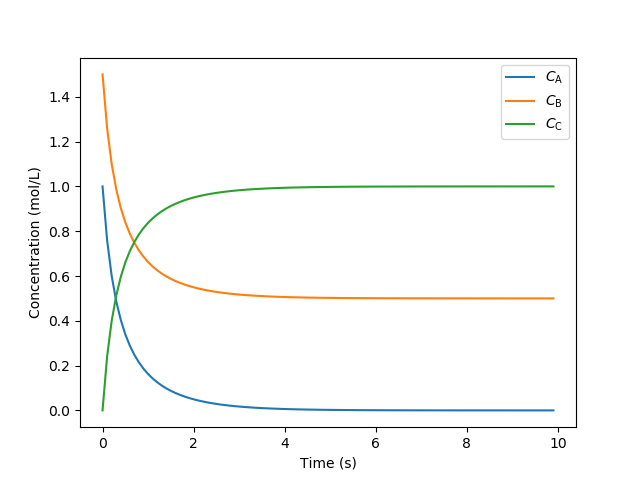
\includegraphics[width=.9\linewidth]{./conc.png}
\end{center}

\section{Analyzing reactor data}
\label{sec:orgf6bbcc2}
\begin{enumerate}
\item Differential methods
\begin{enumerate}
\item Measuring rates
\end{enumerate}
\item Integral methods
\item Half-lives
\end{enumerate}


\begin{minted}[frame=lines,fontsize=\scriptsize,linenos]{python}
import numpy as np               #this lets up handles arrays of data
import matplotlib.pyplot as plt
from scipy.optimize import curve_fit

def differential(x, k, alpha):
    return k*x**alpha

def integral(t, a, b):
    return (2*a/(2+a*b*t))**2

t = np.array([0.00, 2.25, 4.50, 6.33, 8.00, 10.25, 12.00, 13.50, 15.60, 17.85, 19.60, 27.00, 30.00, 38.00, 41.00, 45.00, 47.00, 57.00, 63.00])

C_Br2 = np.array([0.3335, 0.2965, 0.2660, 0.2450, 0.2255, 0.2050, 0.1910, 0.1794, 0.1632, 0.1500, 0.1429, 0.1160, 0.1053, 0.0830, 0.0767, 0.0705, 0.0678, 0.0553, 0.0482])

plt.figure()
plt.plot(t,C_Br2,'o')
plt.xlabel('Time (s)')
plt.ylabel('Concentration (mol/L)')
plt.legend()
plt.savefig('./xylene-conc.png')

delta_t = np.ediff1d(t)        # finite difference between adjacent points
delta_C = np.ediff1d(C_Br2)

grad_t = np.gradient(t)            # second order approximation to gradient, allowing for unequal step size
grad_C = np.gradient(C_Br2)
rate = -np.divide(grad_C,grad_t)

plt.figure()
plt.plot(C_Br2,rate,'o')
plt.xlabel('Concentration (mol/L)')
plt.ylabel('Rate (mol/L/x)')
plt.legend()

popt, pcov = curve_fit(differential, C_Br2, rate )

print('k = {0:f}, alpha={1:f}'.format(popt[0],popt[1]))

model = differential(C_Br2,popt[0],popt[1])
plt.plot(C_Br2,model,'-')

plt.savefig('./xylene-rate.png')

difference_array = np. subtract(rate, model)
squared_array = np. square(difference_array)
mse = squared_array. mean()
print(mse)

# Suggests order of 1.5
popt1, pcov1 = curve_fit(integral, t, C_Br2)
print('k = {0:f}'.format(popt[1]))

model1 = integral(t, popt1[0], popt1[1])

plt.figure()
plt.plot(t,C_Br2,'o')
plt.plot(t,model1,'-')
plt.xlabel('Time (s)')
plt.ylabel('Concentration (mol/L)')
plt.legend()
plt.savefig('./xylene-int-model.png')


\end{minted}

\begin{verbatim}
k = 0.085277, alpha=1.450860
2.4942019231742367e-07
k = 1.450860
\end{verbatim}



\begin{center}
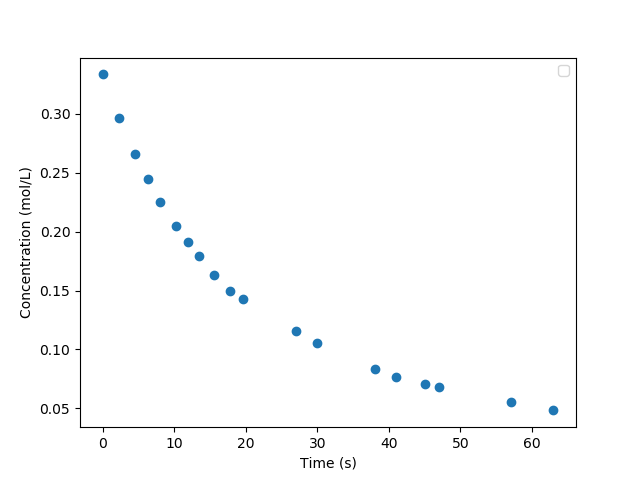
\includegraphics[width=.9\linewidth]{./xylene-conc.png}
\end{center}
\begin{center}
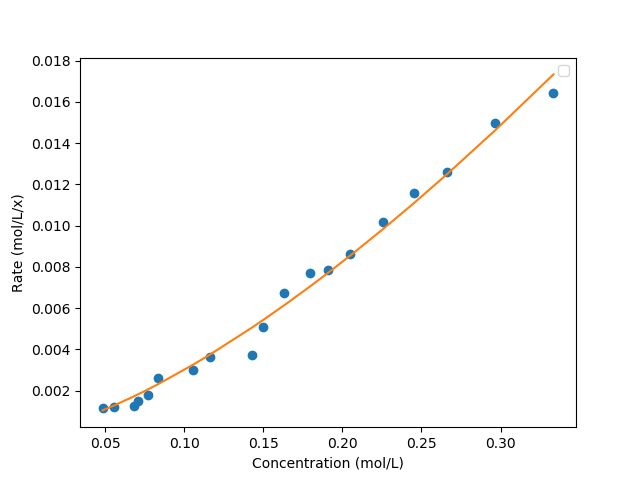
\includegraphics[width=.9\linewidth]{./xylene-rate.png}
\end{center}
\begin{center}
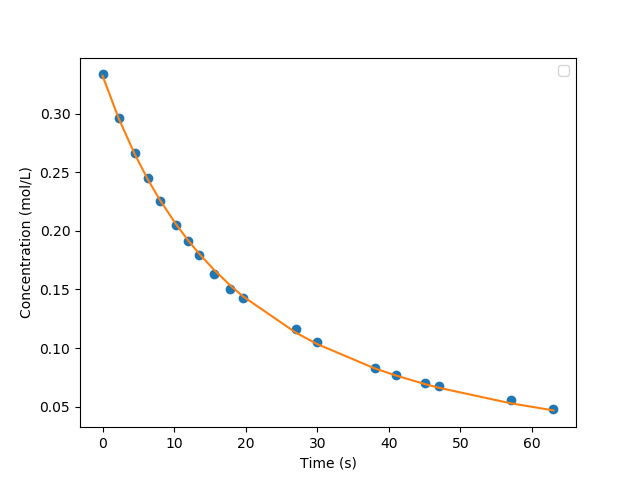
\includegraphics[width=.9\linewidth]{./xylene-int-model.png}
\end{center}

\section{Molecular basis}
\label{sec:orgad7f78d}
\begin{enumerate}
\item reaction pathway, detailed balance
\item bimolecular, collision theory, TST
\item unimolecular reactions
\end{enumerate}

\section{Chemical kinetics}
\label{sec:org30fd904}
\subsubsection{Reaction mechanisms}
\label{sec:org2185406}
\begin{enumerate}
\item Elementary steps and molecularity
\item Ozone decomposition, rate second-order at high \(P_{\ce{O2}}\), first-order at low \(P_{\ce{O2}}\)
\begin{center}
\begin{tabular}{l}
\ce{2 O3 -> 3 O2}\\
\hline
\ce{O3 ->[k_1] O2 + O}\\
\ce{O2 + O ->[k_-1] O3}\\
\ce{O + O3 ->[k_2] 2 O2}\\
\end{tabular}
\end{center}
\item Detailed balance and microscopic reversibility
\item Equilibrium requirement \(K_{eq}(T) = k_f(T)/k_r(T)\)
\item Reversibility \(r_\text{net} = r_f ( 1 - \beta)\), \(\beta = Q/K_c = exp(-\Delta G(T,c_j)/RT)\)
\item Collision theory
\begin{enumerate}
\item A + B \(\rightarrow\) products
\item rate proportional to A/B collision frequency \(z_{AB}\) weighted by fraction of collisions with energy \(> E_a\)
\begin{displaymath}
   r = k C_A C_B , k = \left ( \frac{8 k_B T}{\pi \mu} \right )^{1/2} \sigma_{AB} N_{av} e^{-E_a/k_BT}
\end{displaymath}
\item upper bound on real rates
\end{enumerate}
\end{enumerate}
\subsubsection{Transition state theory (TST)}
\label{sec:org0216821}
\begin{enumerate}
\item Assumptions
\begin{enumerate}
\item Existence of reaction coordinate (PES)
\item Existence of dividing surface
\item Equilibrium between reactants and ``transition state''
\item Harmonic approximation for transition state
\end{enumerate}
\item rate proportional to concentration of ``activated complex'' over reactants times crossing frequency
\begin{eqnarray*}
   r & = & k C_AC_B \\
     & = & k^\ddagger C_{AB}^\ddagger \\
     & = & \nu^\ddagger K^\ddagger C_A C_ B \\
     & = & \nu^\ddagger \frac{k_BT}{h\nu^\ddagger}\bar{K}^\ddagger(T) C_A C_B \\
     & = & \frac{k_B T}{h} \frac{q^\ddagger(T)}{q_A(T) q_B(T)}  e^{-{\Delta E(0)/k_BT}} C_A C_B
\end{eqnarray*}
\item application to atom - atom collision
\item application to two molecules - vinyl alcohol to acetaldehyde
\end{enumerate}

\begin{center}
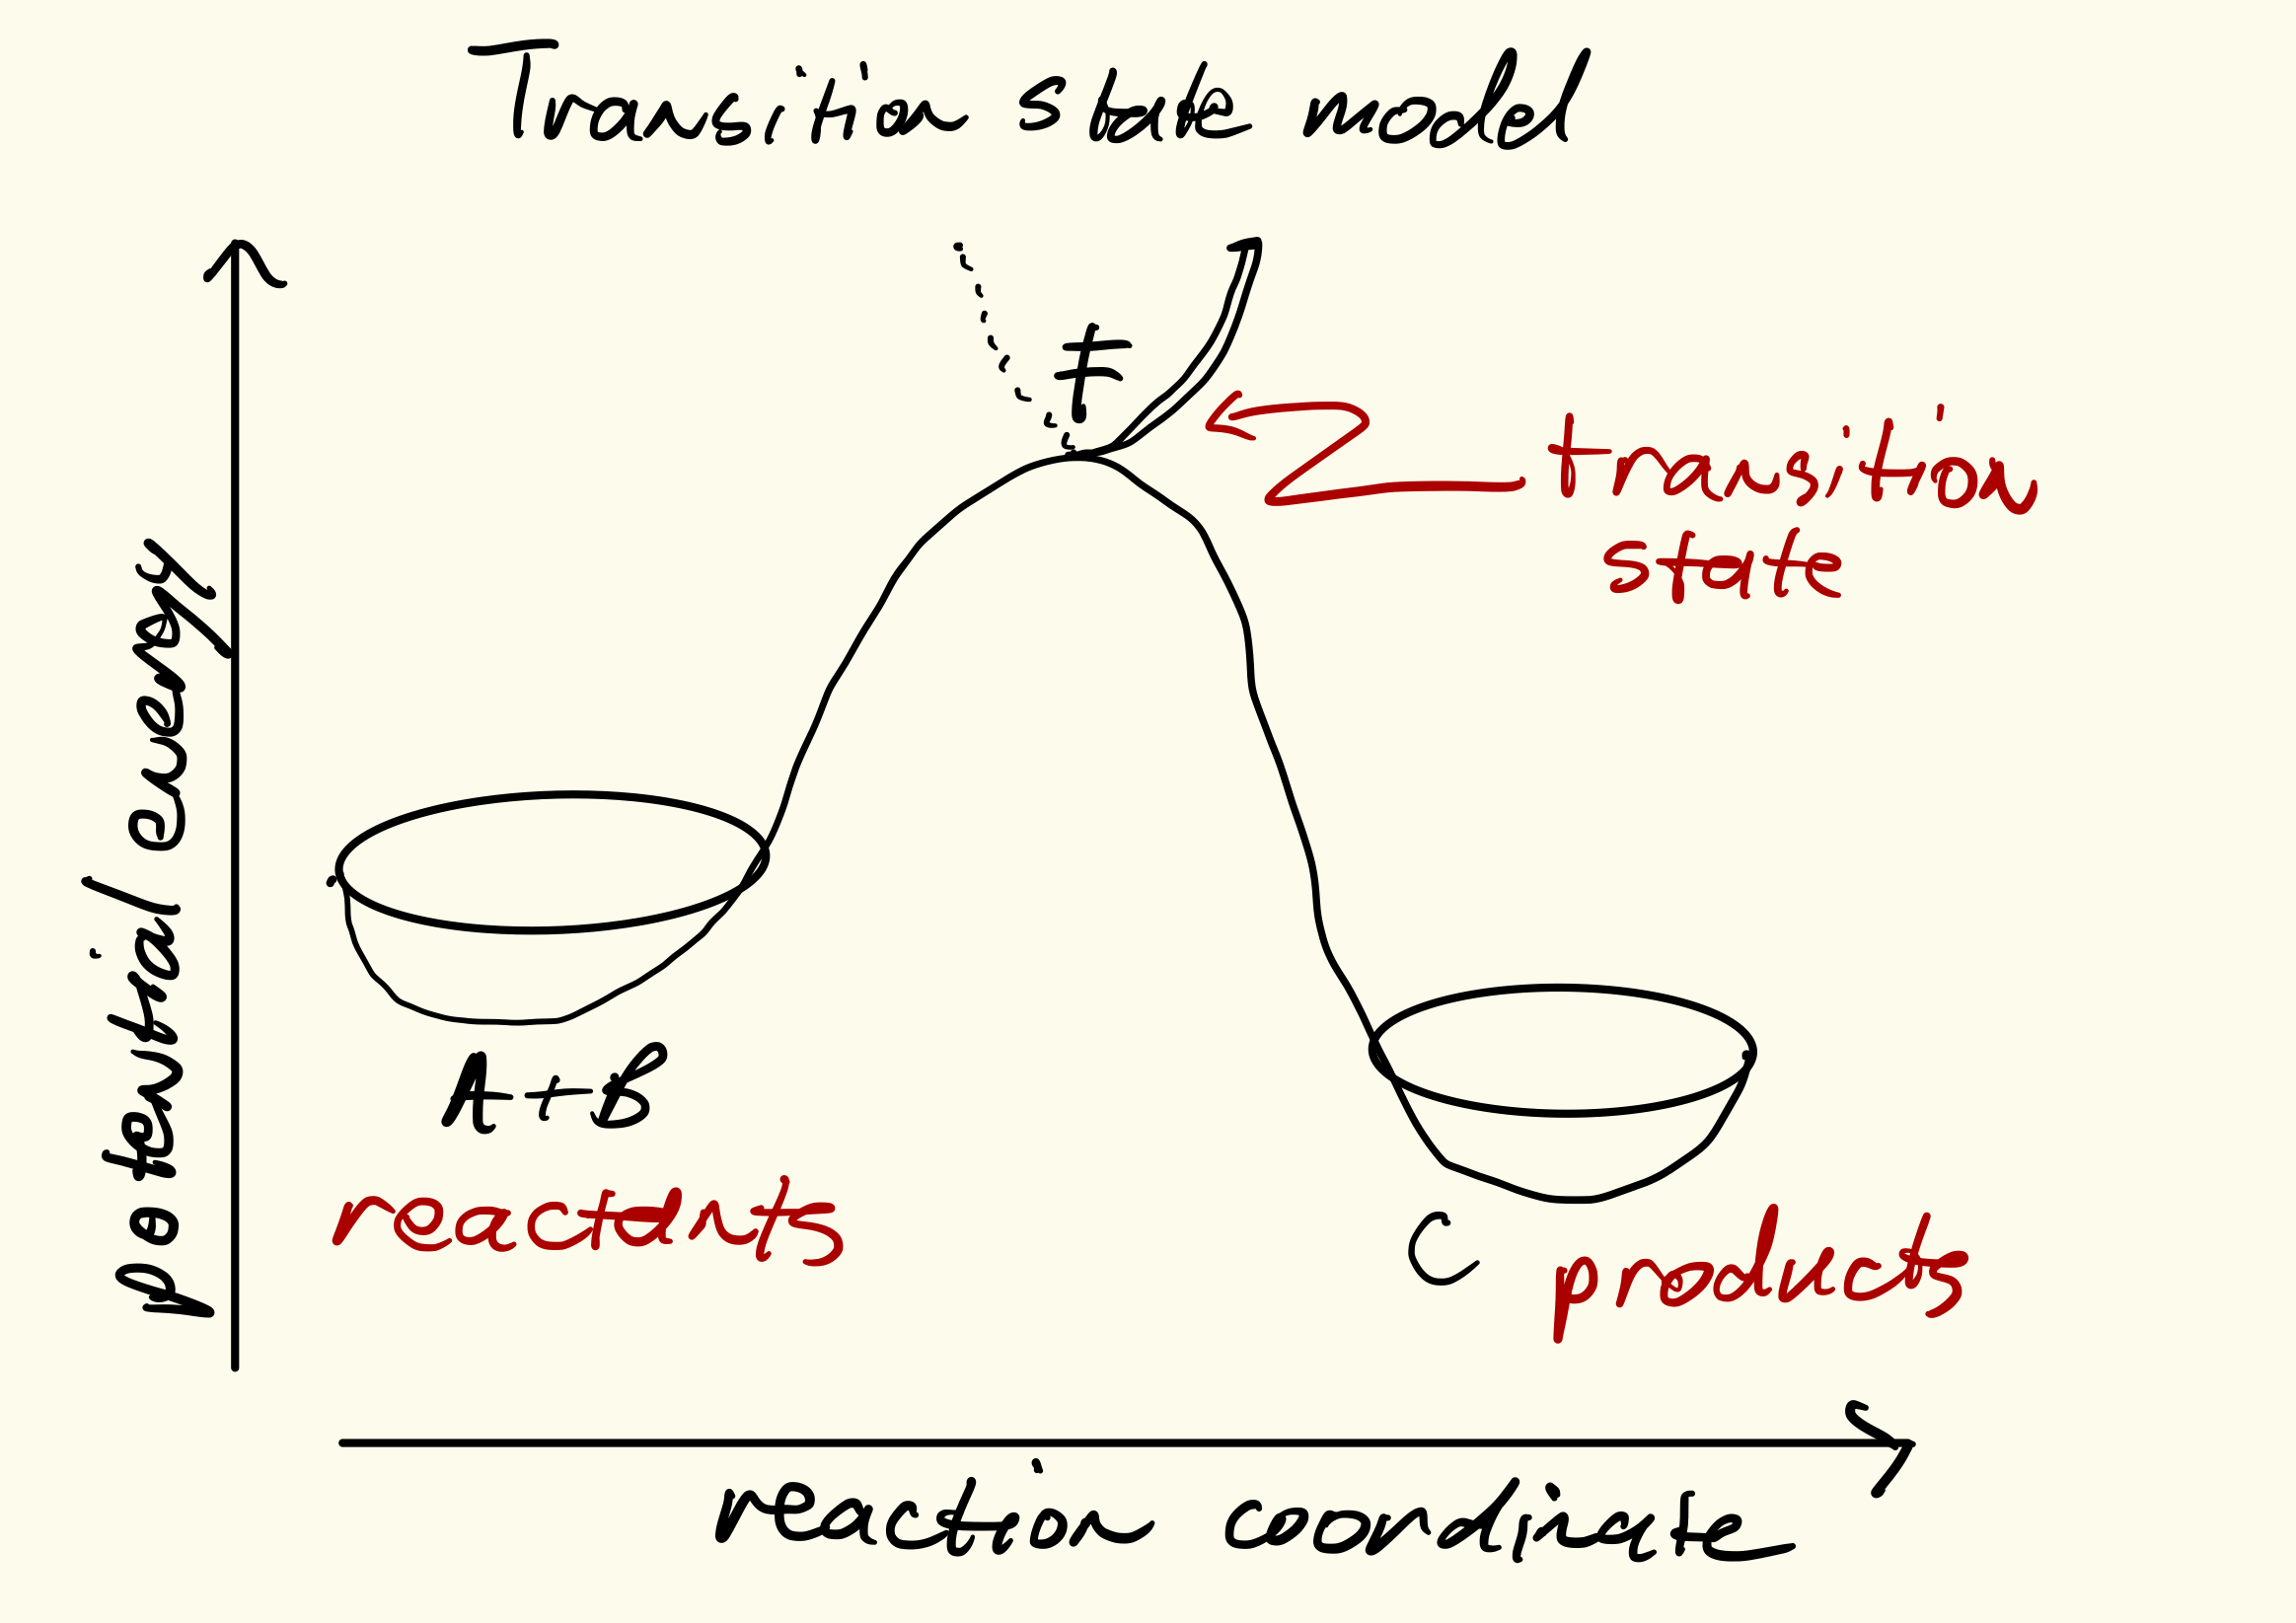
\includegraphics[width=0.6\textwidth]{./Images/PES.png}
\end{center}
\subsubsection{Locating transition states computationally}
\label{sec:org5d44e05}
\subsubsection{Thermodynamic connection}
\label{sec:orga80665e}
\begin{enumerate}
\item Relate activated complex equilibrium constant to activation free energy
\[ \(\bar{K}^\ddagger(T) = e^{-\Delta G^{\circ \ddagger}(T)/kT} = e^{-\Delta H^{\circ \ddagger}(T)/k_BT}e^{\Delta S^{\circ \ddagger}(T)/k_B} \]
\item Compare to Arrhenius expression 
\[E_a = \Delta H^{\circ \ddagger}(T) + kT, A = \frac{k_B T}{h}e^1e^{\Delta S^{\circ \ddagger}(T)/k_B}\]
\end{enumerate}

\begin{verbatim}
Vinyl alcohol to TS  216 kJ/mol
Delta Uddagger (1000 K) =  211 kJ/mol
Delta Addagger (1000 K) =  226 kJ/mol
Delta Sddagger (1000 K) = -1480 J/mol K
\end{verbatim}


\begin{center}
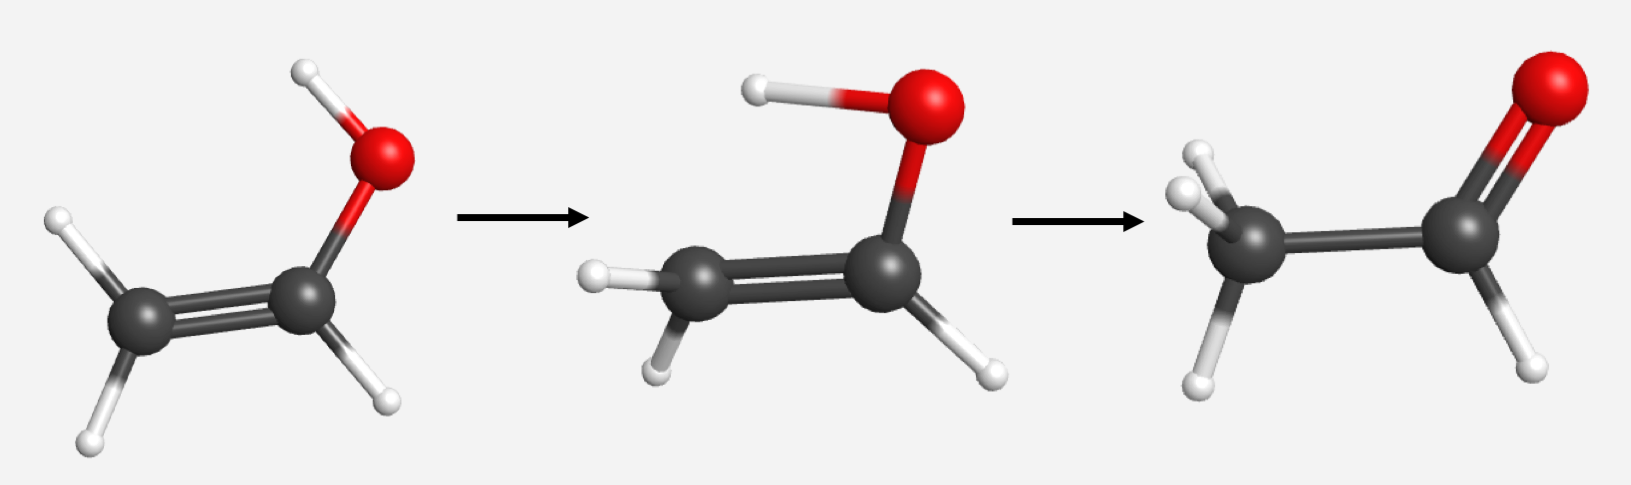
\includegraphics[width=.9\linewidth]{./Images/Path.png}
\end{center}

\begin{center}
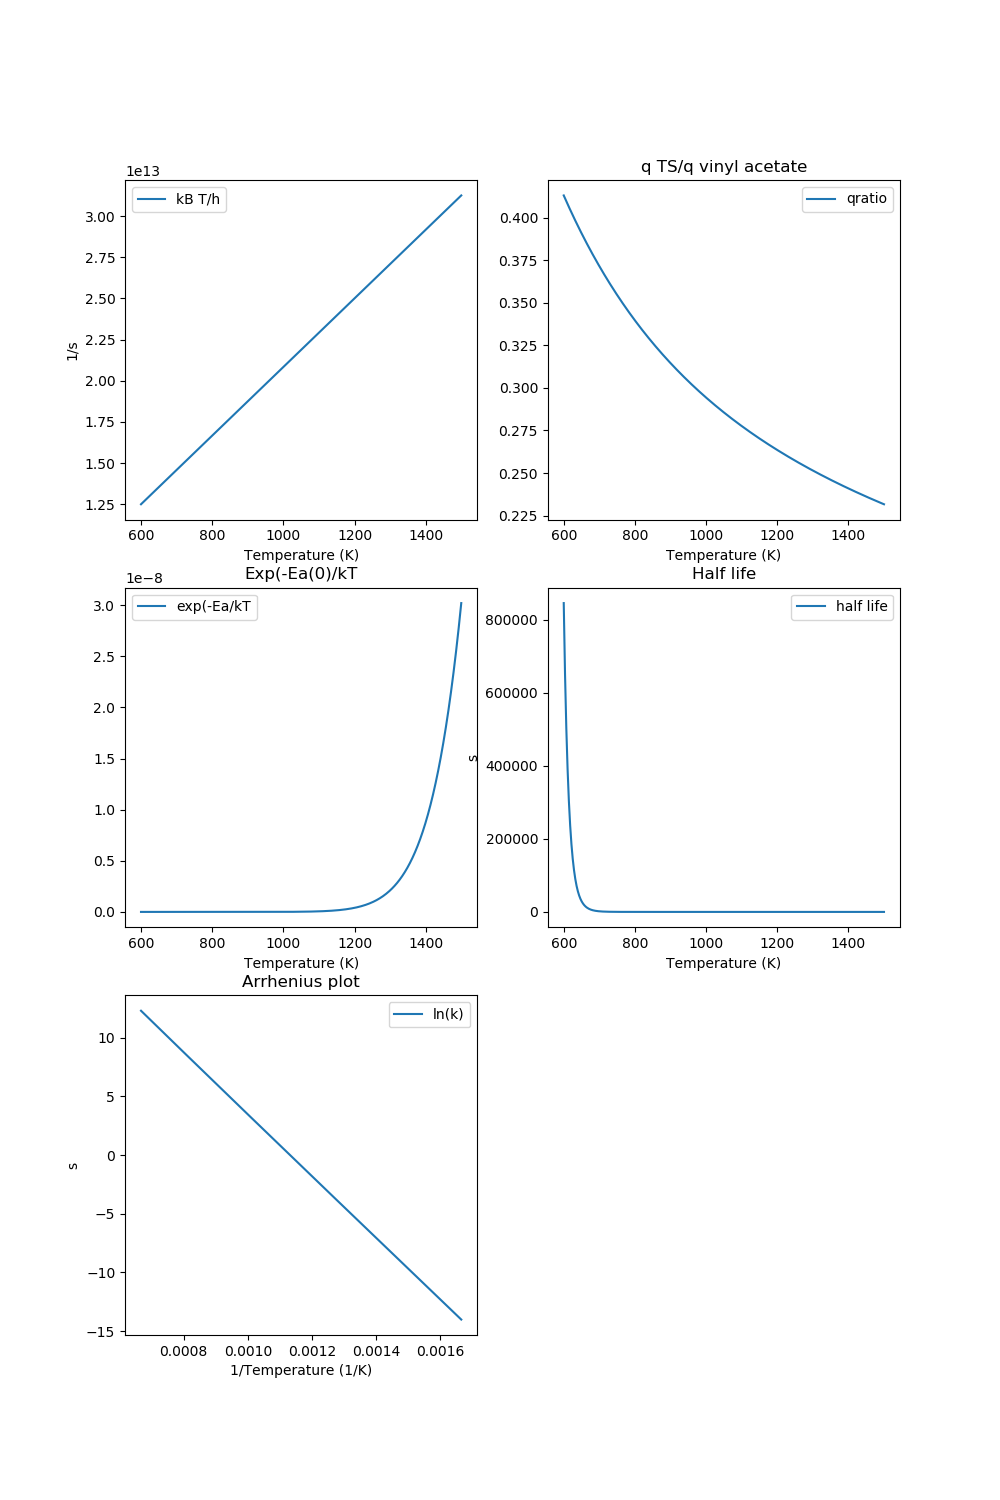
\includegraphics[width=.9\linewidth]{./Images/arrhenius.png}
\end{center}
\begin{center}
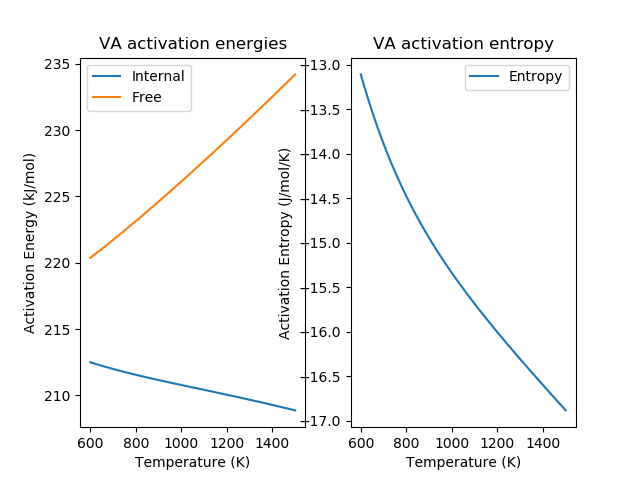
\includegraphics[width=.9\linewidth]{./Images/Sact.png}
\end{center}


\begin{table}
   \caption{Vinyl alcohol to acetaldehyde}
\begin{tabular}{cc}
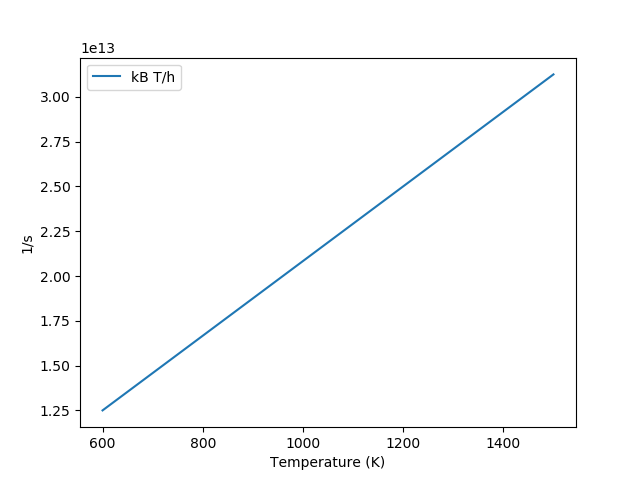
\includegraphics[scale=0.5]{./Images/kTh.png} & 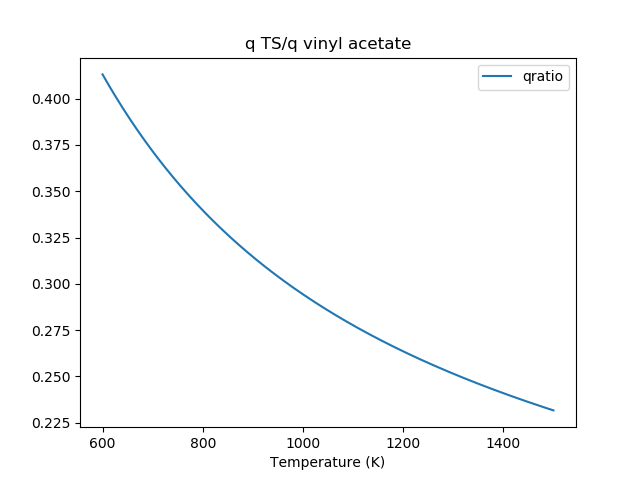
\includegraphics[scale=0.5]{./Images/qratio.png} \\ 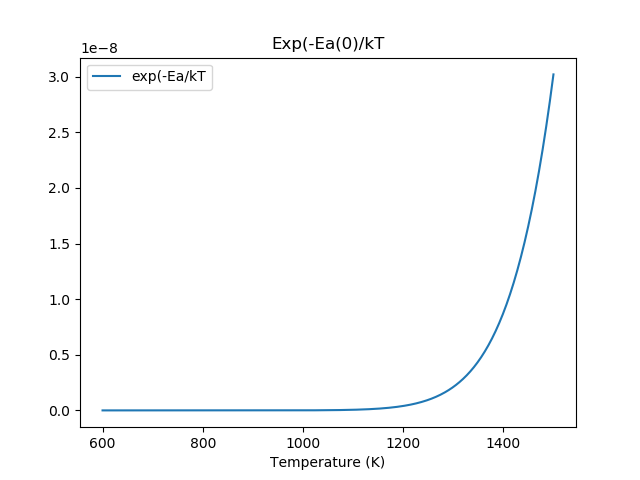
\includegraphics[scale=0.5]{./Images/expEa.png} & 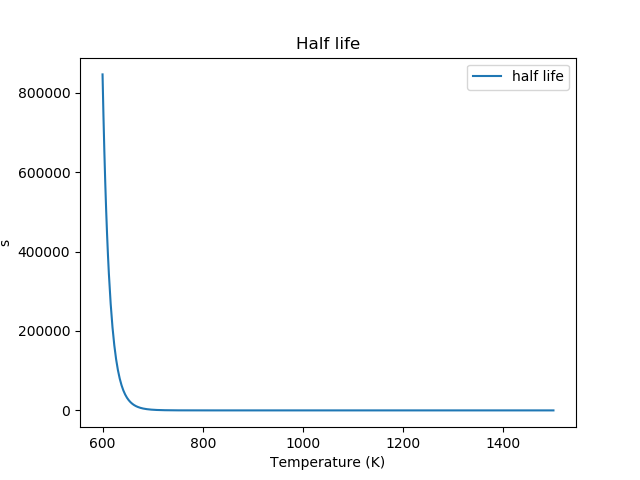
\includegraphics[scale=0.5]{./Images/halflife.png} \\
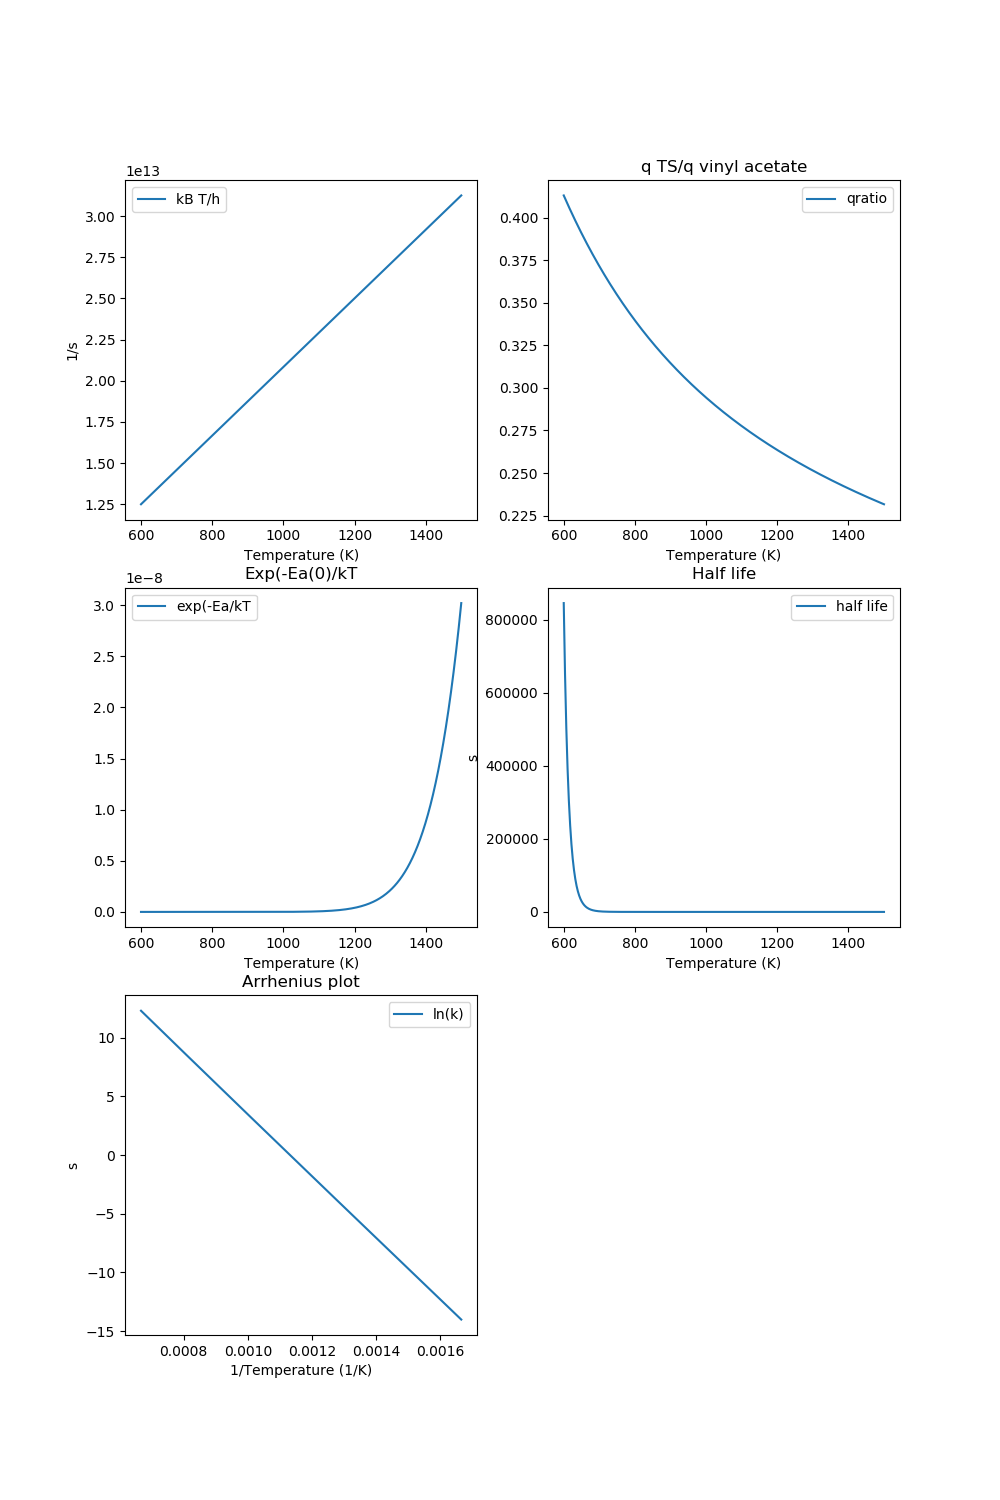
\includegraphics[scale=0.5]{./Images/arrhenius.png} & 
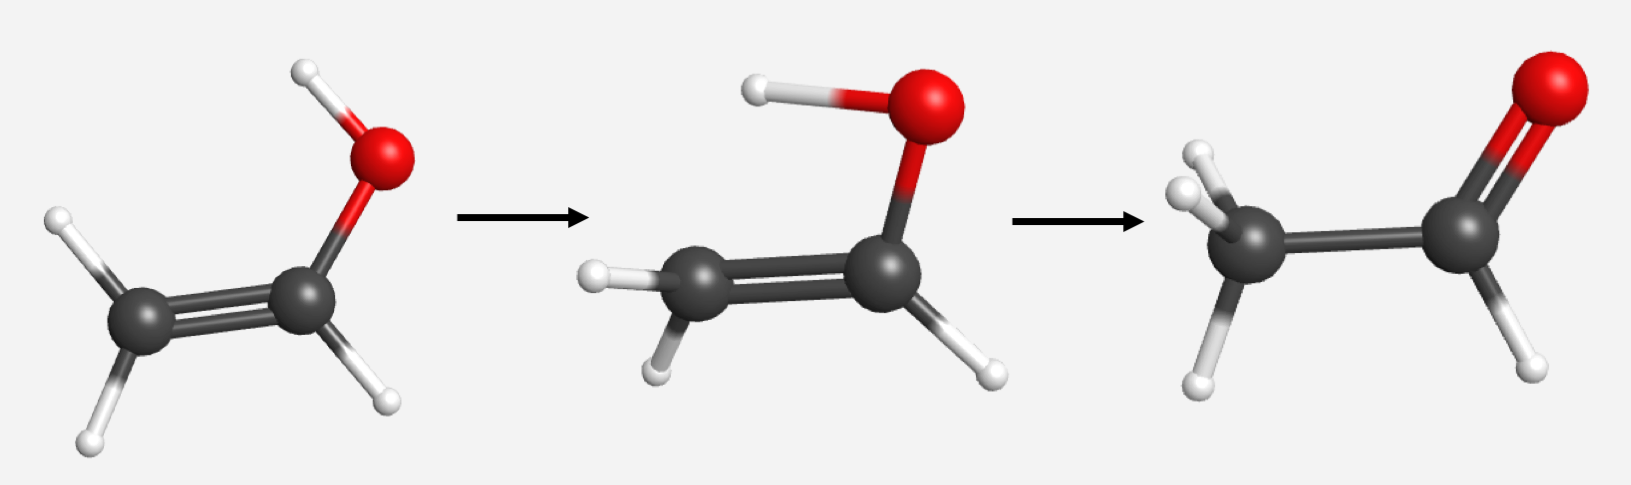
\includegraphics[scale=0.3]{./Images/Path.png} 
\end{tabular}
\end{table}

\subsubsection{Application: gas-phase reactions}
\label{sec:org9bd80a7}
\begin{enumerate}
\item Ethane pyrolysis, \ce{C2H6 -> C2H4 + H2}, \href{https://pubs.acs.org/doi/10.1021/jp206503d}{doi:10.1021/jp206503d}
\end{enumerate}

\section{Mechanisms}
\label{sec:org434f07e}
\begin{enumerate}
\item simple reaction network
\item free energy surface
\item QSSA
\item Pre-equilibrium
\item Selectivity
\item Rate control
\end{enumerate}

\section{Heterogeneous reactions}
\label{sec:org96649f9}
\begin{enumerate}
\item adsorption, L-H
\item TPD
\item catalysis
\item Sabatier analysis
\end{enumerate}
\subsubsection{Heterogeneous reactions and catalysis}
\label{sec:orgdfc3168}
\begin{enumerate}
\item molecule-surface collisions
\item surface reactions
\item Ammonia oxidation, \ce{NH3 + O2 -> NO, N2}, \href{http://pubs.acs.org/doi/10.1021/acscatal.8b04251}{doi:10.1021/acscatal.8b04251}
\end{enumerate}

\begin{table}
   \caption{DFT PES for ethylene dissociation on Ni2P}
\begin{tabular}{cc}
\includegraphics[scale=0.33]{./Images/ethylene-001.png} & \includegraphics[scale=0.33]{./Images/ethylene-002.png} \\ \includegraphics[scale=0.33]{./Images/ethylene-003.png} & \includegraphics[scale=0.33]{./Images/ethylene-004.png} \\
\includegraphics[scale=0.33]{./Images/ethylene-005.png} & 
\includegraphics[scale=0.18]{./Images/ethylene-pes-animation.png} 
\end{tabular}
\end{table}

\url{./Images/TS-Ethylene.gif}

\section{Liquid-phase reactions}
\label{sec:org9997614}
\subsubsection{Diffusion-controlled reactions}
\label{sec:org1a5a973}
\begin{enumerate}
\item Intermediate complex
\item Steady-state approximation
\item Diffusion-controlled limit (\(k_D = 4\pi (r_A + r_B) D_{AB}\))
\item Reaction-controlled limit (\(k_{app}=(k_D/k_{-D})k_r\))
\end{enumerate}

\begin{table}
\begin{center}
    \caption{\large{Equilibrium and Rate Constants}}
   \begin{description}
   \item[Equilibrium Constants] $a~\text{A} + b~\text{B} \rightleftharpoons c~\text{C} + d~\text{D} $
     \begin{eqnarray*}
       K_{eq}(T) &=& e^{\Delta S^\circ(T)/k_B}e^{-\Delta H^\circ(T)/k_BT}
       \\ \\
            K_c(T) &=&
          \left(\frac{1}{c^\circ}\right)^{\nu_c+\nu_d-\nu_a-\nu_b}\frac{(q_c/V)^{\nu_c}(q_d/V)^{\nu_d}}{(q_a/V)^{\nu_a}(q_b/V)^{\nu_b}}e^{-\Delta
            E(0)\beta}\\ \\
            K_p(T) &=&
          \left(\frac{k_BT}{P^\circ}\right)^{\nu_c+\nu_d-\nu_a-\nu_b}\frac{(q_c/V)^{\nu_c}(q_d/V)^{\nu_d}}{(q_a/V)^{\nu_a}(q_b/V)^{\nu_b}}e^{-\Delta
            E(0)\beta}
\end{eqnarray*}
\item[Unimolecular Reaction] $\text[A] \rightleftharpoons [\text{A} ]^\ddagger
  \rightarrow C$
      \begin{displaymath}
        k(T)=\nu^\ddagger \bar K^\ddagger=\frac{k_B T}{h} \frac{\bar{q}_\ddagger(T)/V}{q_A(T)/V}
          e^{-\Delta E^\ddagger(0)\beta}
      \end{displaymath}
\begin{center}
      \begin{tabular}{cc}
      $ \displaystyle E_a =\Delta H^{\circ\ddagger}+k_B T $
      & $ \displaystyle A = e^1\frac{k_B T}{h} e^{\Delta S^{\circ\ddagger}} $
      \end{tabular}
\end{center}
\item[Bimolecular Reaction] $
        \mathrm{A} + \mathrm{B} \rightleftharpoons [ \mathrm{AB}]^\ddagger
        \rightarrow \text{C}$
      \begin{displaymath}
        k(T)=\nu^\ddagger \bar K^\ddagger=\frac{k_B T}{h} \frac{q_\ddagger(T)/V}{(q_A(T)/V)(q_B(T)/V)}\left
          (\frac{1}{c^\circ}\right )^{-1}
        e^{-\Delta E^\ddagger(0)\beta}
      \end{displaymath}
      \begin{center}
        \begin{tabular}{cc}
        $ \displaystyle E_a  =\Delta H^{\circ\ddagger}+2 k_B T $ & $ \displaystyle
        A  = e^2\frac{k_B T}{h} e^{\Delta S^{\circ\ddagger}} $
      \end{tabular}
      \end{center}
   \end{description}
 \end{center}
 \end{table}
\end{document}